\chapter{基于消息传递网络的复合物筛选模型}
\label{chapter:MPNN}
\section{引言}
\label{section:MPNN:Put}

模型\ref{section:NodeConv:intro}和模型\ref{section:EdgeConv:intro}分别是结点嵌入和邻边嵌入模型,蛋白质复合物的形成和蛋白质以及蛋白质互作相关。
普通的GCN模型只能将邻边特征转换为结点特征之后再进行图卷积运算,这个过程将邻边特征均匀的分配给了其相邻的结点,在模型训练过程中不再将邻边作为独立的计算元素。这种情形下,邻边特征只能作为结点特征的补充,无法与复合物互作网络动态的结合起来。

为了将邻边特征与结点特征整合到模型的动态参数更新中,本节基于消息传递网络(Message Passing Neural Network,简称MPNN)提出蛋白质复合物特征融合模型,同时处理蛋白质复合物子图中的结点数据和邻边数据,将生物数据、全局拓扑特征以及局部拓扑特征动态的融合起来。
\section{消息传递网络介绍}
\label{section:MPNN:intro}



\section{基于消息传递网络的复合物筛选模型}
\label{section:MPNN:detail}

融合模型是基于MPNN网络的改进,MPNN网络是一种基于消息传递的图结构学习框架,不同于图卷积模型必须将特征绑定到结点,MPNN将图结构的特征当成消息,特征在结构中的流动被视为消息的传递。在此框架下,图卷积神经网络可以被当作MPNN的特例,是只传递结点消息的MPNN网络。
MPNN网络的具体实现如式\ref{equ:MPNNPassing}所示。

\begin{equation}
    \label{equ:MPNNPassing}
    m_v^{t+1} = \sum_{w \in N_{(v)}}M_t(h_v^t,h_w^t,e_{vw}^t)
\end{equation}

\begin{equation}
    \label{equ:MPNNReadout}
    h_v^{t+1} = U_t(h_v^t,m_v^{t+1})
\end{equation}
其中$N_{(v)}$表示图中结点$v$的邻居,$t$为时间步。公式\ref{equ:MPNNPassing}表示消息传递阶段(Message Passing),$M_t$表示消息传递的更新函数,代表结点w向结点v传递消息的过程中,其传递的消息$h_v^t,h_w^t,e_{vw}$的更新方式。公式\ref{equ:MPNNReadout}表示更新阶段,$U_t$表示更新阶段的函数,代表结点v汇总所有周围消息后的数据更新方式。

为了使得结点特征和邻边特征具有融合的能力,蛋白质复合物特征融合模型中采用了结点更新邻边,邻边更新结点的方式。在每一层的MPNN过程中,结点t时刻特征更新为邻边t+1时刻特征、邻边t特征更新为结点t+1时刻特征。结点特征的更新具体方法如下所示,其中$Linear$为一层感知器。
\begin{equation}
    \label{equ:MineMPNNPassing}
    m_v^{t+1} = \sum_{w \in N_{(v)}}Linear^t(e_{vw}^t)
\end{equation}

\begin{equation}
    \label{equ:MineMPNNReadout}
    h_v^{t+1} = Max(h_v^t,m_v^{t+1})
\end{equation}
从式中可以看出,结点的特征更新来源分为两部分,其一为汇聚所有邻边的特征$e_{vw}^t$,同时为了保留一部分结点中具有关键性的原始特征,其更新方式采用了maxpool。邻边特征的具体更新方法如下所示。
\begin{equation}
    \label{equ:MineMPNNedge}
    e_{vw}^{t+1} = Max(e_{vw}^t,Linear_0^t(m_w^{l} - m_v^{l}) + Linear_1^t m_v^{l})
\end{equation}
从式中得出,类似于结点更新模型,邻边的特征更新也可以分为两部分,最后同样采用了maxpool的方式保留关键邻边特征。邻边特征的更新方式综合考虑了源点到汇点的特征流动部分$m_w^{l} - m_v^{l}$以及汇点的特征保留部分$m_v^{l}$。


最后融合模型同样考虑了复合物子图的整体拓扑特征,为通过图论计算的总体拓扑结构数据,作为不可学习的特征与MPNN读出的特征拼接到一起,作为最终的图特征输出。总体拓扑特征计算参考\cite{yu_predicting_2014}。

\section{算法具体实现与流程}
\label{section:MPNN:flow}

首先是PPI网络特征融合过程,将GO注释特征、拓扑域特征以及亚细胞定位特征嵌入到PPI网络的邻边中,将Deepwalk特征、GAE特征嵌入到PPI网络的结点中。整个PPI网络此时兼具结点和邻边特征,再在该网络的基础上按照标准集和COACH算法抽取数据集,包括标准集对应的正样本、COACH对应的中间样本和随机的负样本。
\begin{figure}[htbp]
    \centering
    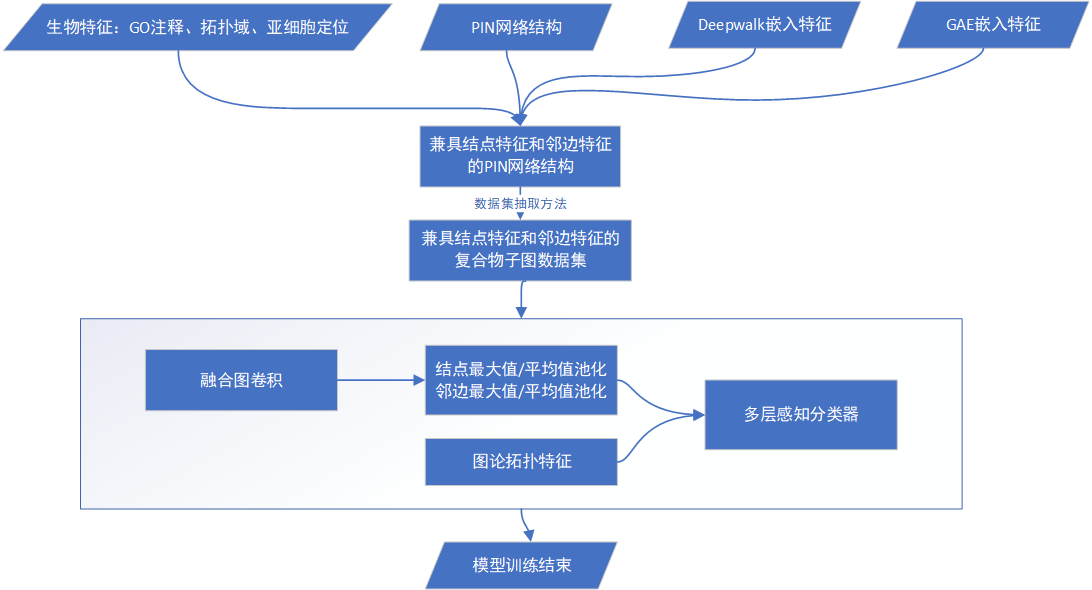
\includegraphics[width=14cm]{fusion-classification-flow}
    \caption{基于特征融合的分类模型总体流程}
    \label{fig:fusion-classification-flow}
\end{figure}

数据集中每一个样本都为蛋白质复合物子图,继承了PPI网络的结点特征和邻边特征。在所有的子图样本上训练蛋白质复合物特征融合模型,层数设置为两层。融合模型的读出阶段同时考虑如下四个方面,结点maxpool、结点meanpool、邻边maxpool以及邻边meanpool,作为子图的可学习特征。后续子图不可学习的拓扑特征和可学习特征拼接到一起,作为最终的子图特征输出。分类阶段采用了两层感知器预测分类结果和评分结果。


\section{实验设计及结果分析}
\label{section:MPNN:experience}
图\ref{fig:result/DIP/fusion}为在DIP网络中,基于结点的全局特征模型、基于邻边的生物特征模型以及特征融合模型筛选之后结果的对比。
\begin{figure}[htbp]
    \centering
    \subcaptionbox{F1值对比}{\label{fig:result/DIP/F1/fusion}
        \includegraphics[width=10cm]{result/DIP/F1/fusion}}
    \vskip0.2cm
    \subcaptionbox{SPA值对比}{\label{fig:result/DIP/SPA/fusion}
        \includegraphics[width=10cm]{result/DIP/SPA/fusion}}
    \caption{DIP网络不同模型处理后结果对比}
    \label{fig:result/DIP/fusion}
\end{figure}

图\ref{fig:result/Biogrid/fusion}为在Biogrid网络中,基于结点的全局特征模型、基于邻边的生物特征模型以及特征融合模型筛选之后结果的对比。
\begin{figure}[htbp]
    \centering
    \subcaptionbox{F1值对比}{\label{fig:result/Biogrid/F1/fusion}
        \includegraphics[width=10cm]{result/Biogrid/F1/fusion}}
    \vskip0.2cm
    \subcaptionbox{SPA值对比}{\label{fig:result/Biogrid/SPA/fusion}
        \includegraphics[width=10cm]{result/Biogrid/SPA/fusion}}
    \caption{Biogrid网络不同模型处理后结果对比}
    \label{fig:result/Biogrid/fusion}
\end{figure}
\section{本章小结}
\label{section:MPNN:summary}